\documentclass[12pt,a4paper]{article}

\usepackage{amsmath,amssymb}
\usepackage{graphicx}
\usepackage{geometry}
\usepackage{hyperref}
\usepackage{float}
\usepackage{listings}
\usepackage{xcolor}

\geometry{margin=1in}

% Code listing settings
\lstset{
    basicstyle=\ttfamily\small,
    breaklines=true,
    frame=single,
    language=Java
}

\title{
\textbf{J2GO: Java to Go Transpiler} \\
\vspace{0.3cm}
\large A Case Study for Theory of Computation and Compiler Design
}

\author{
[Name 1] (Roll No. 1)\\
[Name 2] (Roll No. 2)\\
[Name 3] (Roll No. 3)\\
[Name 4] (Roll No. 4)
}

\date{}

\begin{document}
\maketitle

%------------------------------------------------
\section*{Abstract}

Modern compilers are complex software systems that rely heavily on formal language theory and automata models. This project presents a case study that applies concepts from Automata Theory and Compiler Design to the development of a Java to Go transpiler (J2GO). The compilation process is modeled as a pipeline of automata, transforming the source code through various intermediate representations. Each phase—lexical analysis, syntax analysis, AST traversal, and code generation—is analyzed using Deterministic Finite Automata (DFA) and formal grammars to ensure correctness and efficiency.

%------------------------------------------------
\section*{Problem Statement}

Source-to-source translation requires rigorous formal modeling to ensure that the semantics of the input program are preserved in the output. Ad-hoc translation methods often lead to edge cases and incorrect code generation. This project studies how deterministic finite automata, context-free grammars, and tree automata can be applied to model the transpilation pipeline formally.

%------------------------------------------------
\section*{Objectives}

\begin{itemize}
    \item To model the tokenization of Java source code using Deterministic Finite Automata.
    \item To represent the syntax analysis phase using Pushdown Automata and Context-Free Grammars.
    \item To apply tree automata concepts for Abstract Syntax Tree (AST) traversal and manipulation.
    \item To establish the relevance of Theory of Computation in modern compiler construction.
\end{itemize}

%------------------------------------------------
\newpage

\section*{Automata Theory Modeling}

\subsection*{Notation}

\begin{itemize}
    \item $c$ denotes a character from the source code,
    \item $tok$ denotes a token generated by the lexer,
    \item $node$ denotes a node in the Abstract Syntax Tree.
\end{itemize}

%================================================
\subsection*{DFA 1: Lexical Analysis Architecture}

The DFA for keyword and identifier recognition is defined as:
\[
M_1 = (Q, \Sigma, \delta, q_0, F)
\]

\begin{itemize}
    \item \textbf{State set}
    \[
    Q = \{q_0, q_{\text{letter}}, q_{\text{keyword}}, q_{\text{id}}\}
    \]

    \item \textbf{Alphabet} $\Sigma = \{a\text{-}z, A\text{-}Z, 0\text{-}9, \_ \}$
    \item \textbf{Transition function} $\delta : Q \times \Sigma \rightarrow Q$
    \item \textbf{Initial state} $q_0$
    \item \textbf{Final state set} $F = \{q_{\text{keyword}}, q_{\text{id}}\}$
\end{itemize}

\begin{figure}[H]
\centering
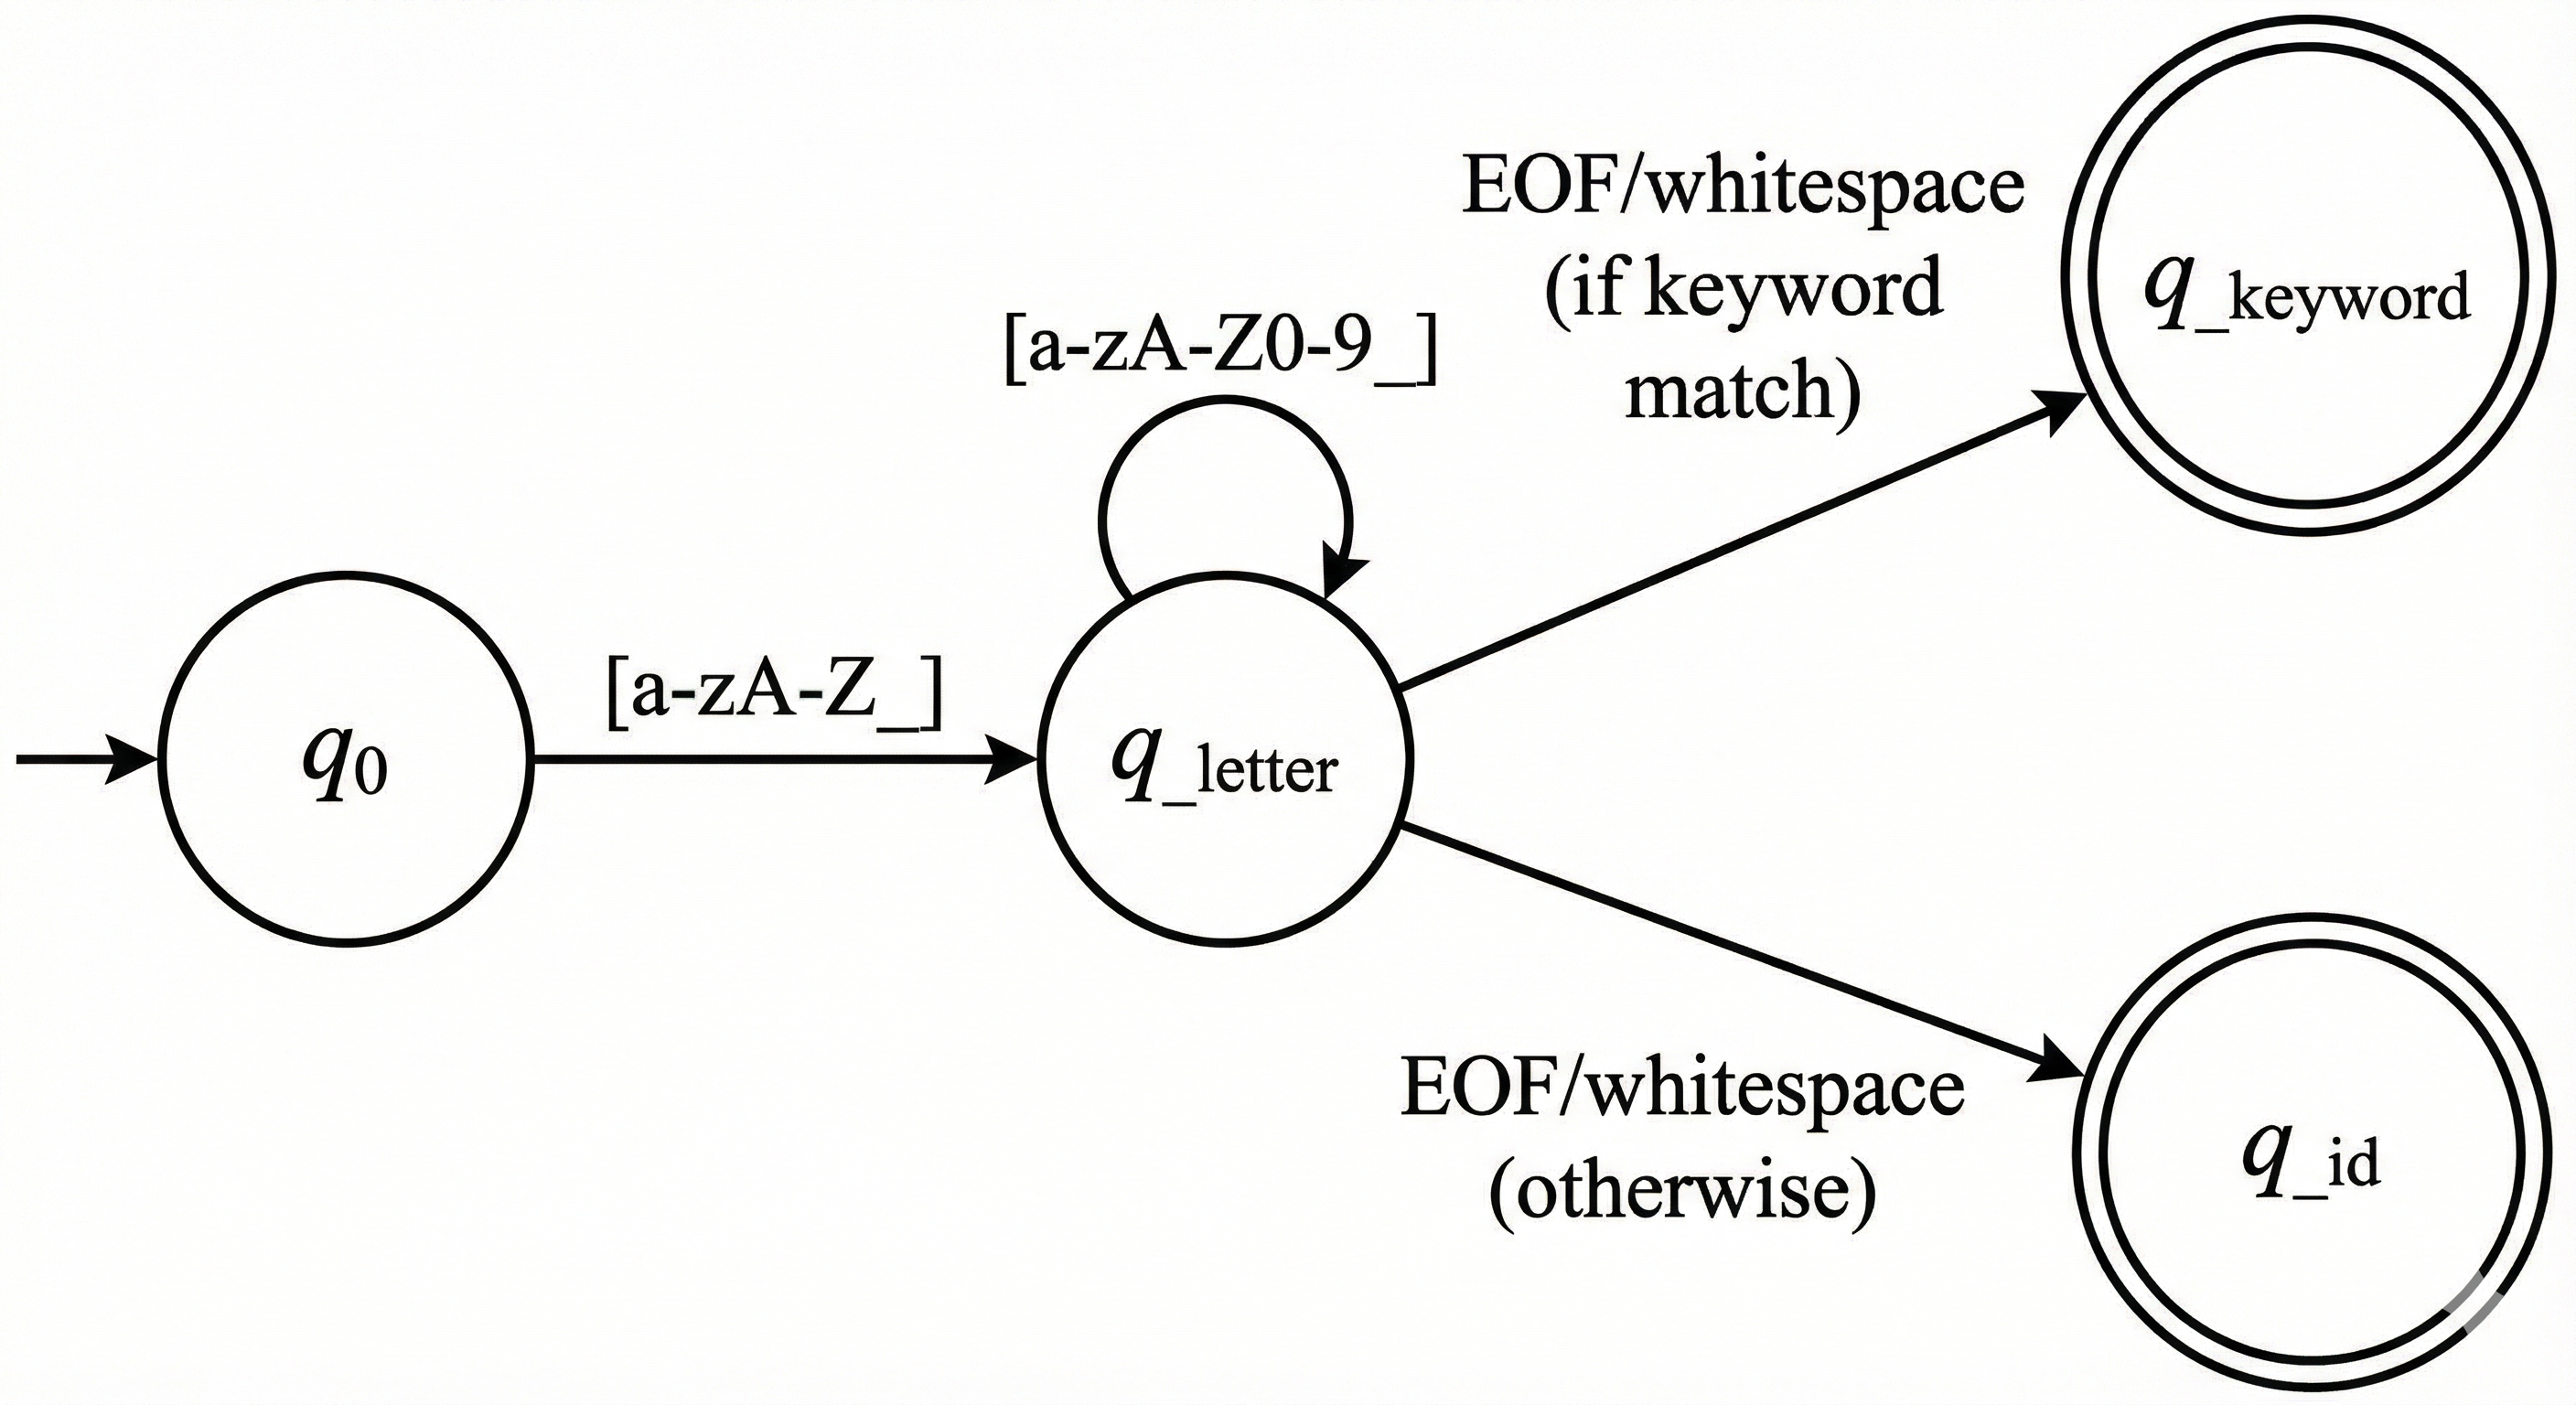
\includegraphics[width=\textwidth]{dfa1_lexer_keyword.png}
\caption{DFA 1: Keyword and Identifier Recognition}
\end{figure}

\subsubsection*{Transition Table}
The transition table explicitly defines the transition function $\delta$ of the DFA, mapping each state and input character to the next state.

\begin{table}[H]
\centering
\begin{tabular}{|c|c|c|}
\hline
Current State & Input & Next State \\
\hline
$q_0$ & [a-zA-Z\_] & $q_{\text{letter}}$ \\
$q_{\text{letter}}$ & [a-zA-Z0-9\_] & $q_{\text{letter}}$ \\
$q_{\text{letter}}$ & EOF/Space & $q_{\text{keyword}}$ or $q_{\text{id}}$ \\
\hline
\end{tabular}
\end{table}

\subsubsection*{Regular Grammar}

The regular grammar for tokens is defined as:

\[
G_1 = (V, T, P, S)
\]

\begin{itemize}
    \item \textbf{Variable set}
    \[
    V = \{S, A, B\}
    \]

    \item \textbf{Terminal set}
    \[
    T = \{a\text{-}z, A\text{-}Z, 0\text{-}9\}
    \]

    \item \textbf{Start symbol} $S$

    \item \textbf{Production rules}
    \[
    S \rightarrow \text{letter} A
    \]
    \[
    A \rightarrow \text{letter} A \mid \text{digit} A \mid \lambda
    \]
\end{itemize}

\subsubsection*{Regular Expression}
The regular expression represents the set of valid identifiers in the language.
\[ L(M_1) = [a\text{-}zA\text{-}Z\_][a\text{-}zA\text{-}Z0\text{-}9\_]* \]

\subsubsection*{Explanation}

This DFA models the lexical analysis phase where raw character streams are converted into meaningful tokens. The state machine transitions based on character classes (letters, digits) to identify keywords and identifiers. This corresponds to the implementation of the `Lexer` class, which uses a maximal munch algorithm to identify the longest matching token.

%================================================
\subsection*{DFA 1.2: Number Literal Recognition}

The DFA for recognizing integer and floating-point literals is defined as:
\[
M_{1.2} = (Q, \Sigma, \delta, q_0, F)
\]

\begin{figure}[H]
\centering
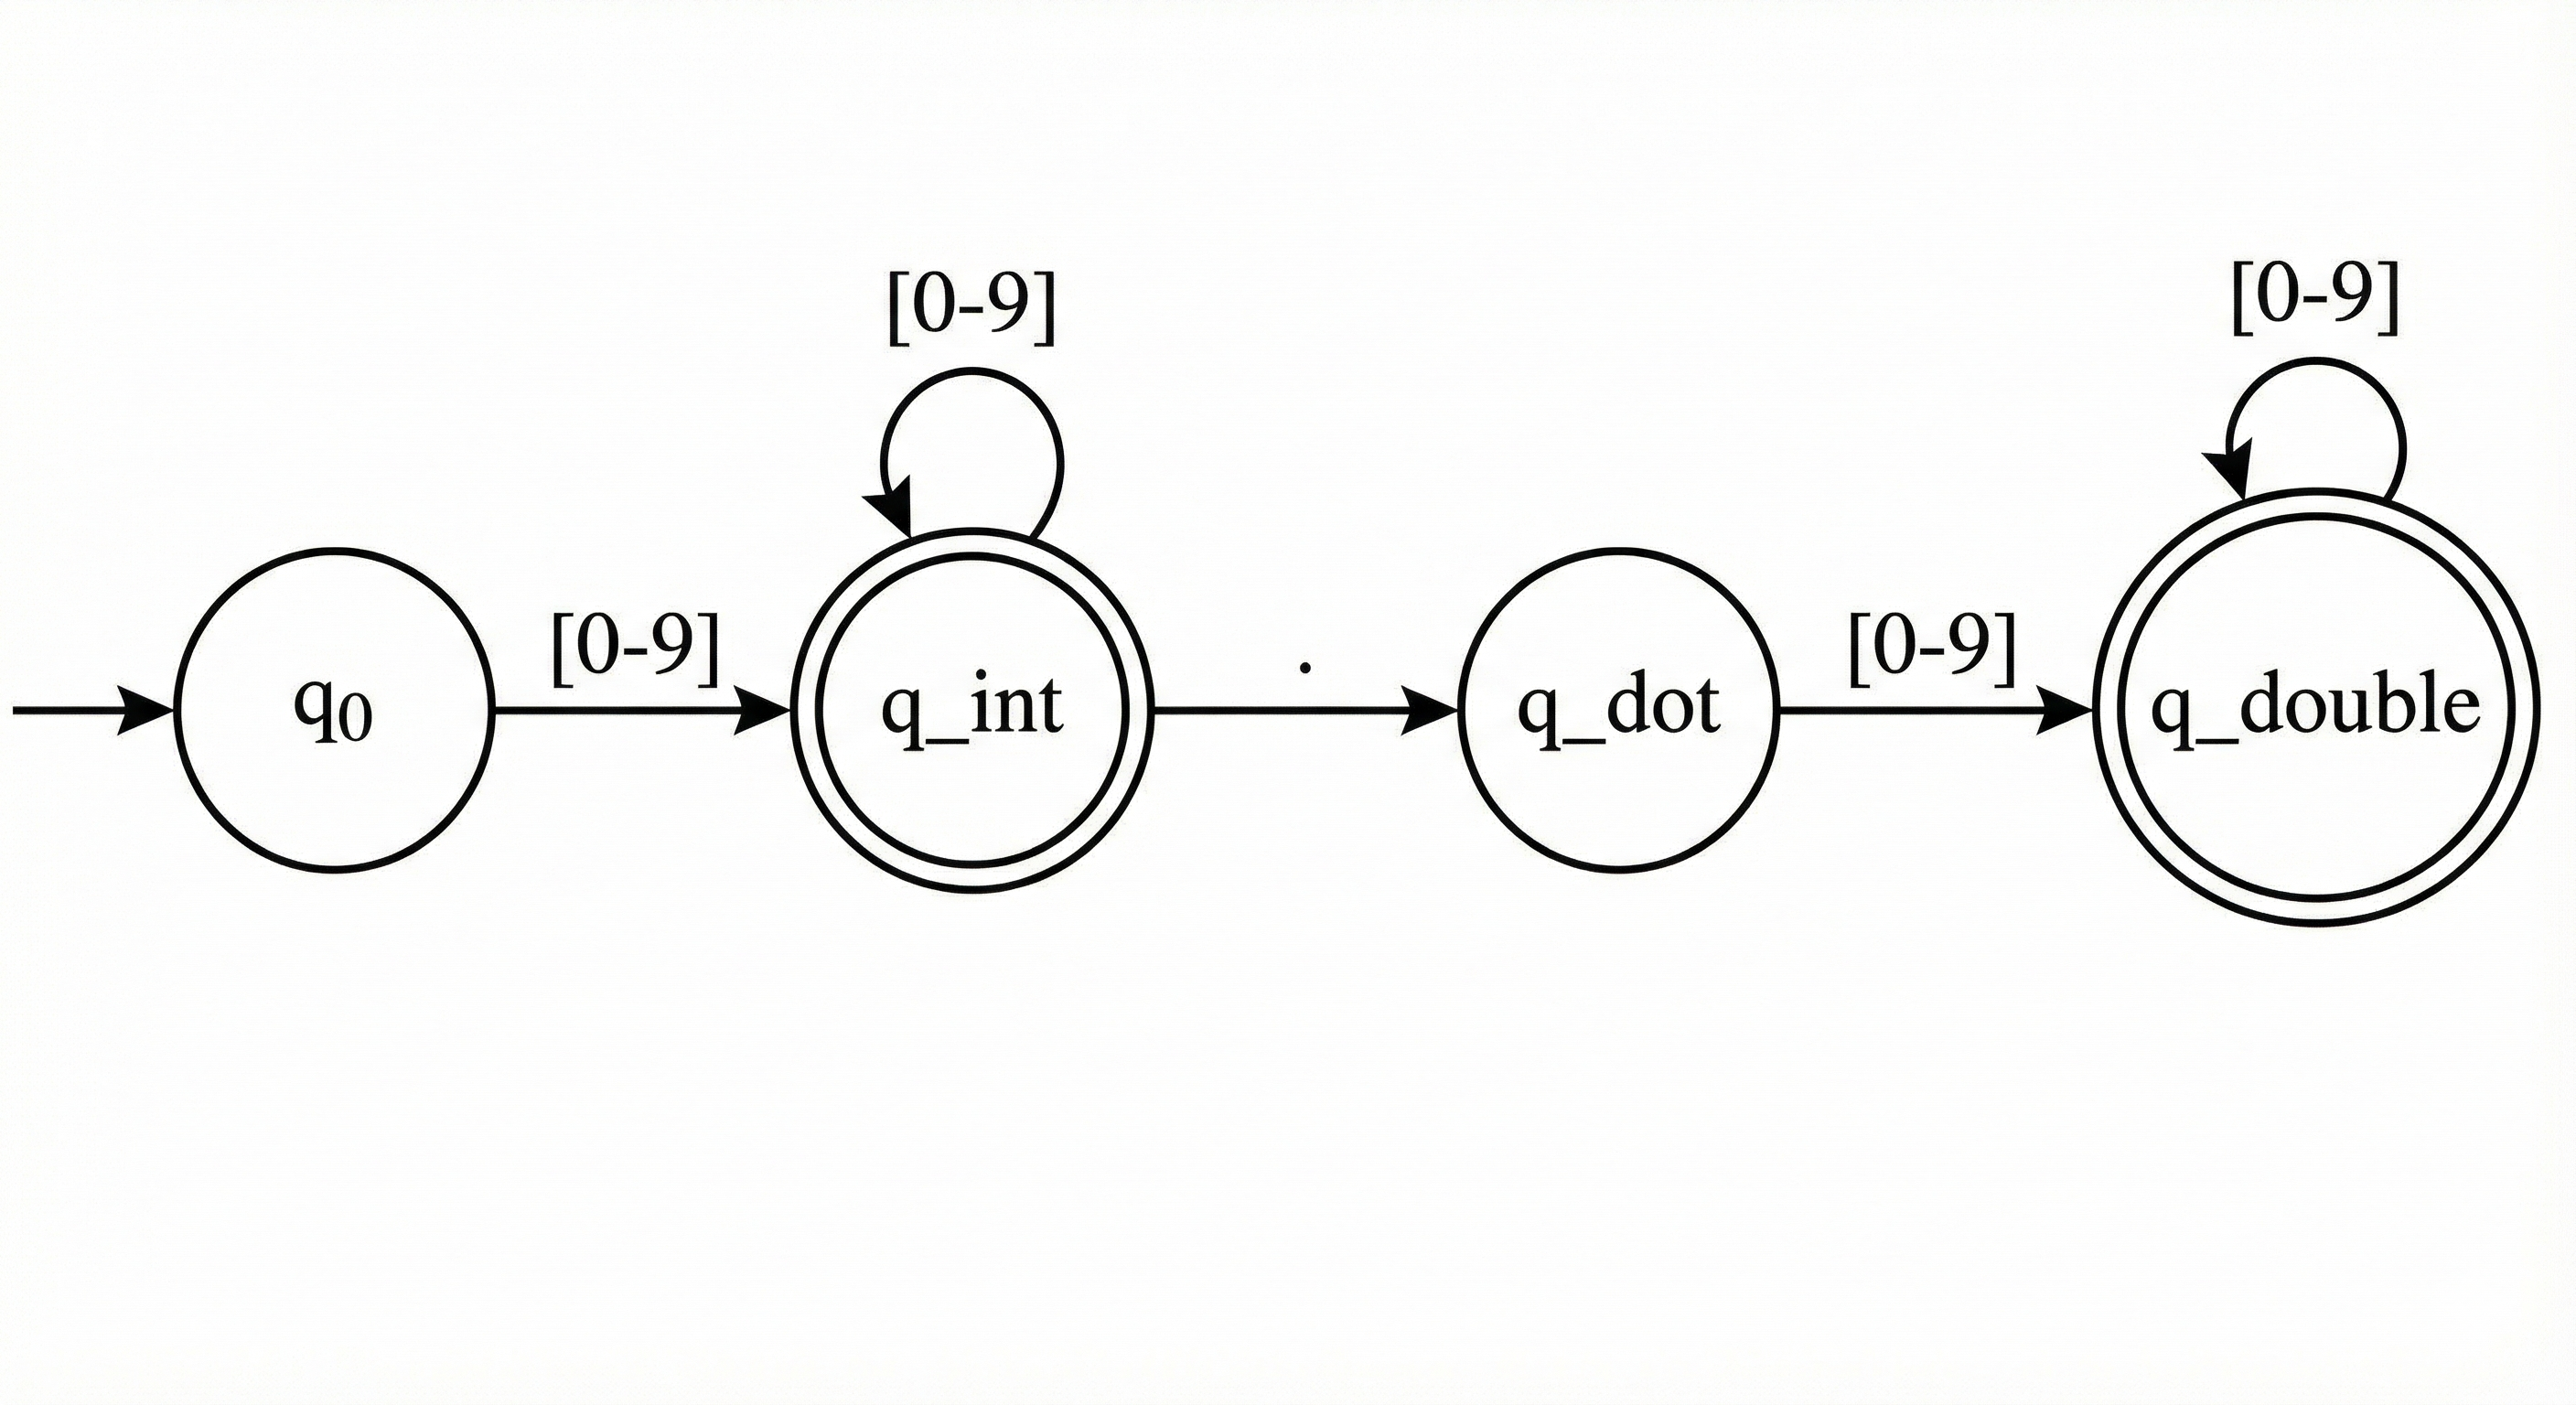
\includegraphics[width=\textwidth]{dfa1b_lexer_number.png}
\caption{DFA 1.2: Number Literal Recognition}
\end{figure}

\subsubsection*{Explanation}
This DFA distinguishes between integer and floating-point literals. It transitions to an integer state upon reading digits. If a decimal point is encountered, it transitions to a state expecting fractional digits, ultimately accepting a double literal.

%================================================
\subsection*{DFA 1.3: Operator Recognition}

The DFA for recognizing single and multi-character operators is defined as:
\[
M_{1.3} = (Q, \Sigma, \delta, q_0, F)
\]

\begin{figure}[H]
\centering
\includegraphics[width=\textwidth]{dfa1c_lexer_operator.png}
\caption{DFA 1.3: Operator Recognition}
\end{figure}

\subsubsection*{Explanation}
This DFA handles the recognition of operators, including multi-character operators like `==`, `!=`, `&&`, and `||`. It uses lookahead to distinguish between assignment (`=`) and equality (`==`), or logical NOT (`!`) and inequality (`!=`).

%================================================
\subsection*{DFA 2: Syntax Analysis Architecture}
The DFA for statement parsing is defined as:

\[
M_2 = (Q, \Sigma, \delta, q_0, F)
\]

\begin{itemize}
    \item \textbf{State set}
    \[
    Q = \{q_{\text{start}}, q_{\text{if}}, q_{\text{while}}, q_{\text{return}}, q_{\text{block}}, q_{\text{expr}}\}
    \]

    \item \textbf{Alphabet} $\Sigma = \{\text{Tokens}\}$

    \item \textbf{Transition function} $\delta : Q \times \Sigma \rightarrow Q$

    \item \textbf{Initial state} $q_0 = q_{\text{start}}$

    \item \textbf{Final state set} $F = \{q_{\text{accept}}\}$
\end{itemize}

\begin{figure}[H]
\centering
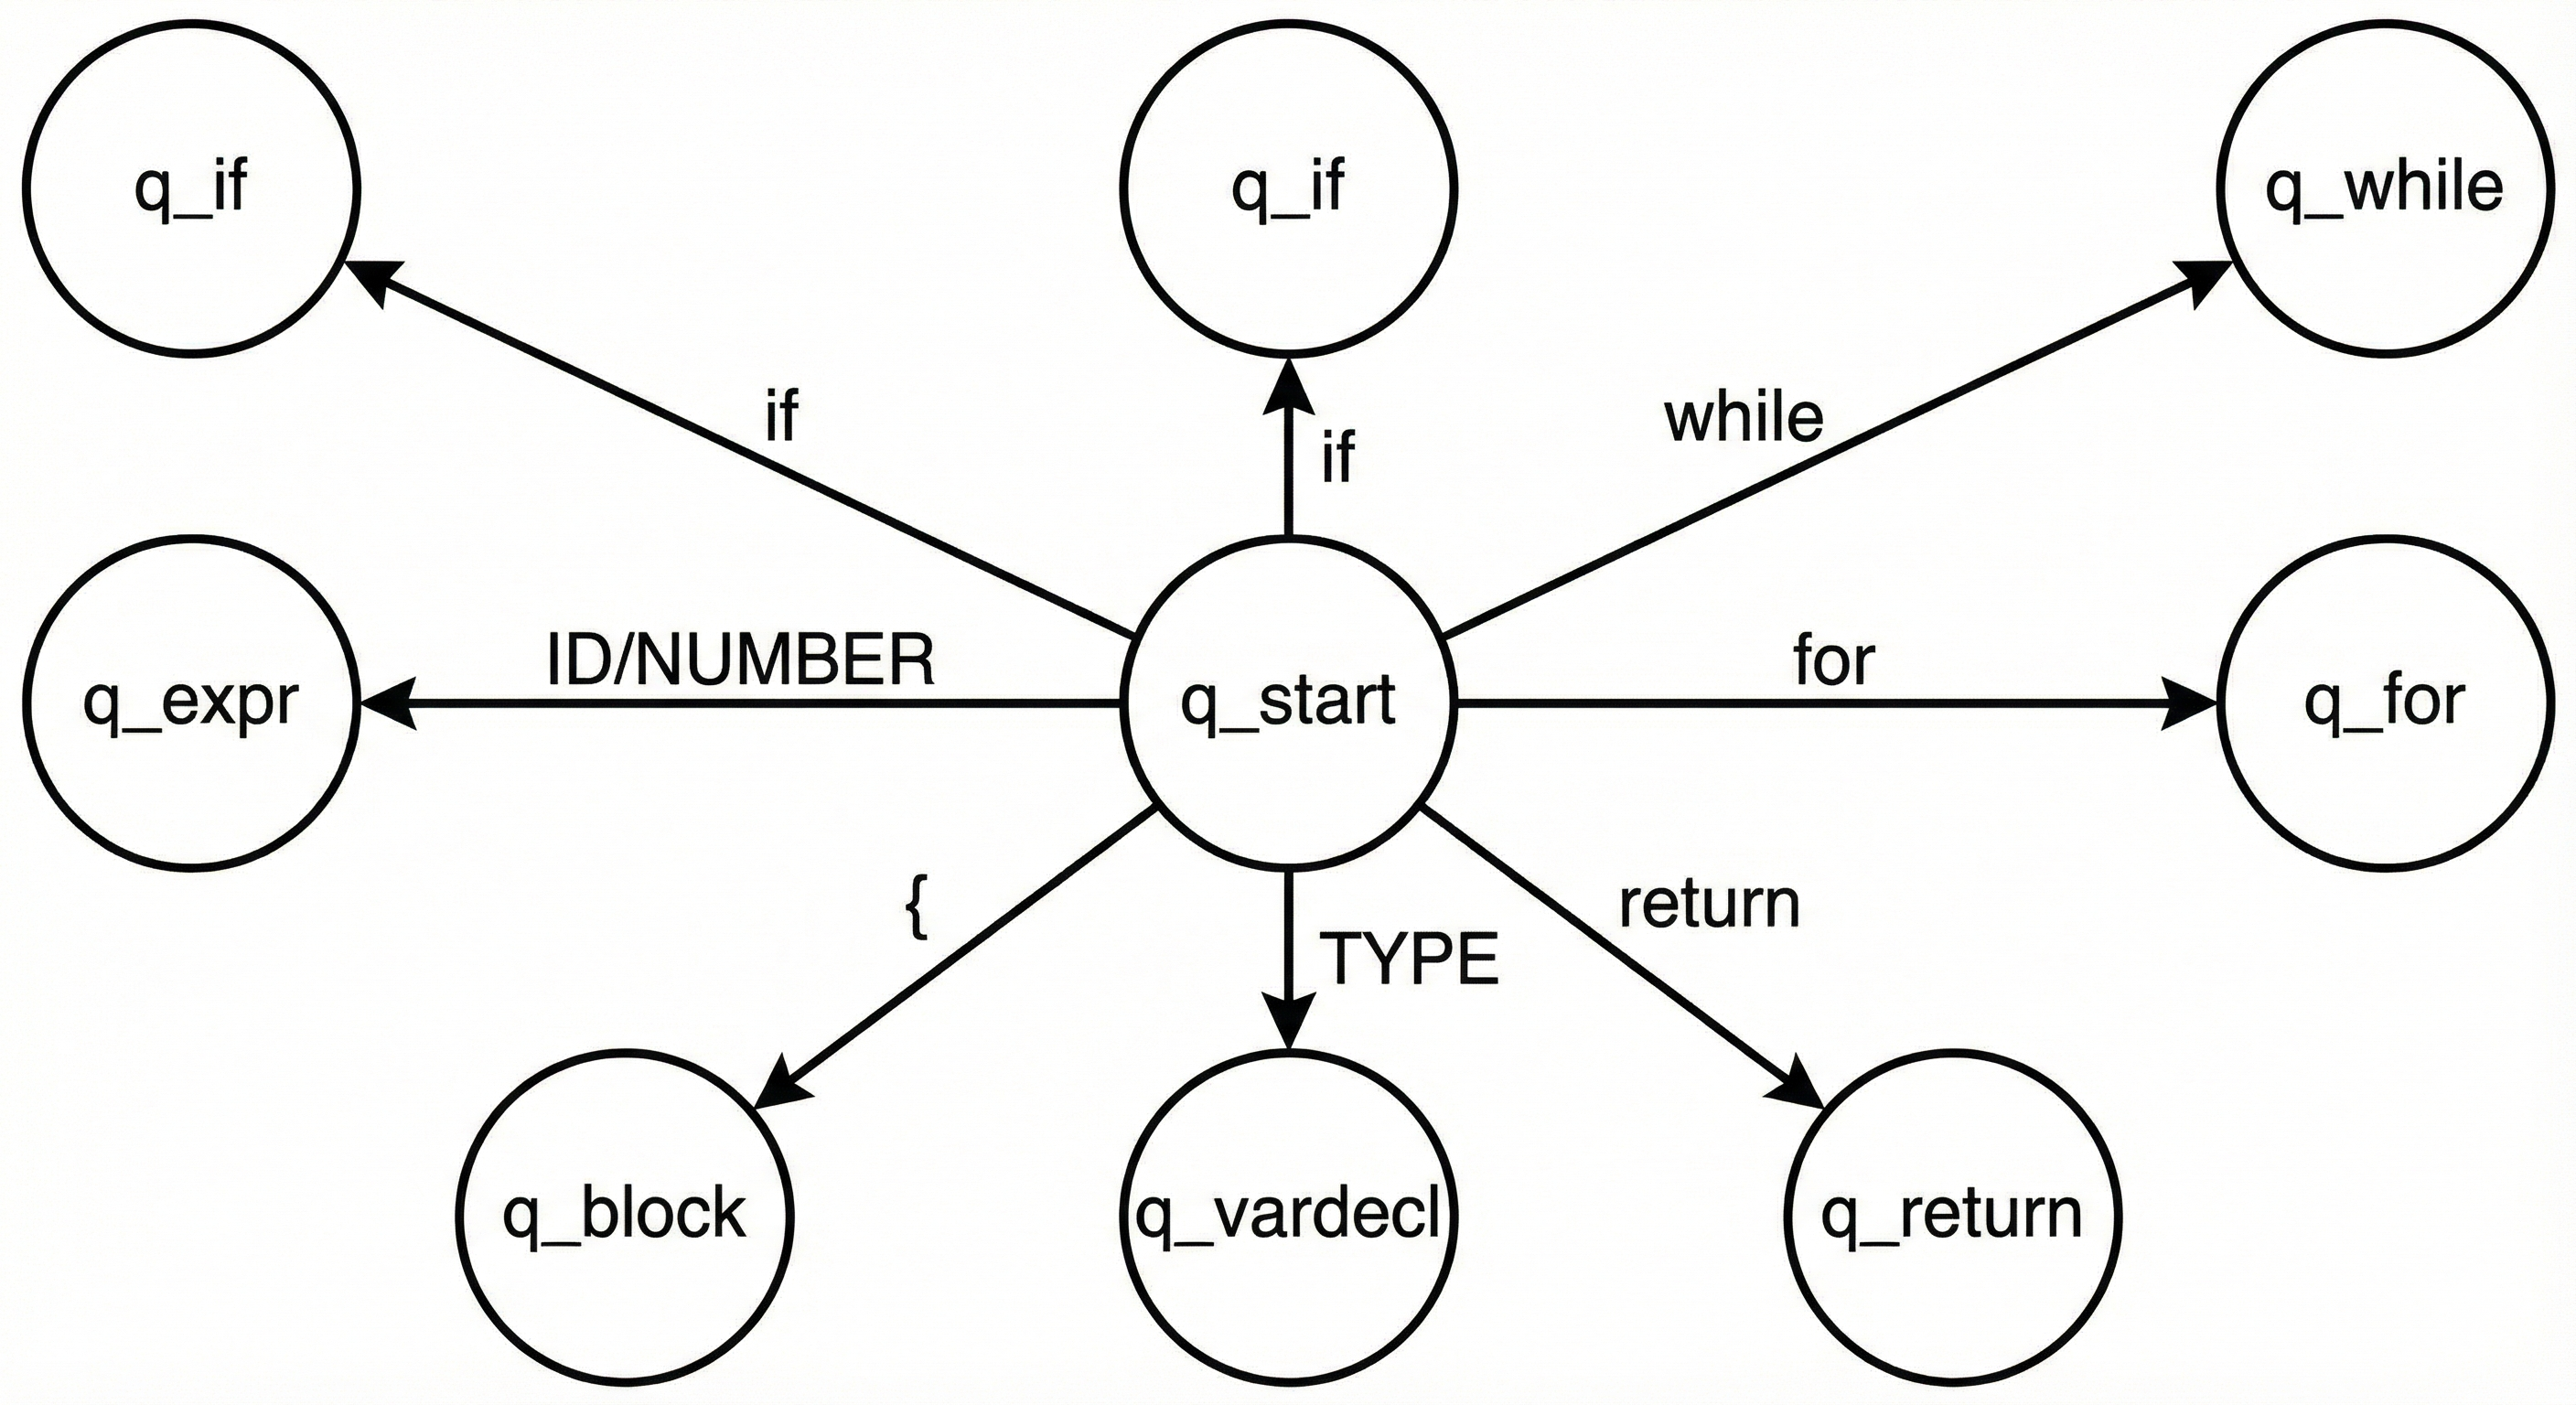
\includegraphics[width=\textwidth]{dfa2_parser_statement.png}
\caption{DFA 2: Statement Parsing State Machine}
\end{figure}

\subsubsection*{Transition Table}

\begin{table}[H]
\centering
\begin{tabular}{|c|c|c|}
\hline
Current State & Input Token & Next State \\
\hline
$q_{\text{start}}$ & if & $q_{\text{if}}$ \\
$q_{\text{start}}$ & while & $q_{\text{while}}$ \\
$q_{\text{start}}$ & return & $q_{\text{return}}$ \\
$q_{\text{start}}$ & \{ & $q_{\text{block}}$ \\
$q_{\text{start}}$ & ID & $q_{\text{expr}}$ \\
\hline
\end{tabular}
\end{table}

\subsubsection*{Context-Free Grammar}

The grammar is defined as:

\[
G_2 = (V, T, P, S)
\]

\begin{itemize}
    \item \textbf{Variable set}
    \[
    V = \{Stmt, IfStmt, WhileStmt, Block, Expr\}
    \]

    \item \textbf{Terminal set} $T = \{if, while, return, \{, \}, ID, ...\}$

    \item \textbf{Start symbol} $Stmt$

    \item \textbf{Production rules}
    \[
    Stmt \rightarrow IfStmt \mid WhileStmt \mid Block \mid Expr ;
    \]
\end{itemize}

\subsubsection*{Explanation}
This DFA represents the control flow of the recursive descent parser. Unlike a standard DFA, this machine operates on a stream of tokens to determine the syntactic structure of the program. It models the decision-making process of the parser: seeing an 'if' token triggers the `parseIfStatement` transition, while a '{' triggers `parseBlock`. This ensures the input program adheres to the defined grammar.

%================================================
\subsection*{Parse Tree Visualization}

The following diagram illustrates the parse tree generated for a variable declaration statement.

\begin{figure}[H]
\centering
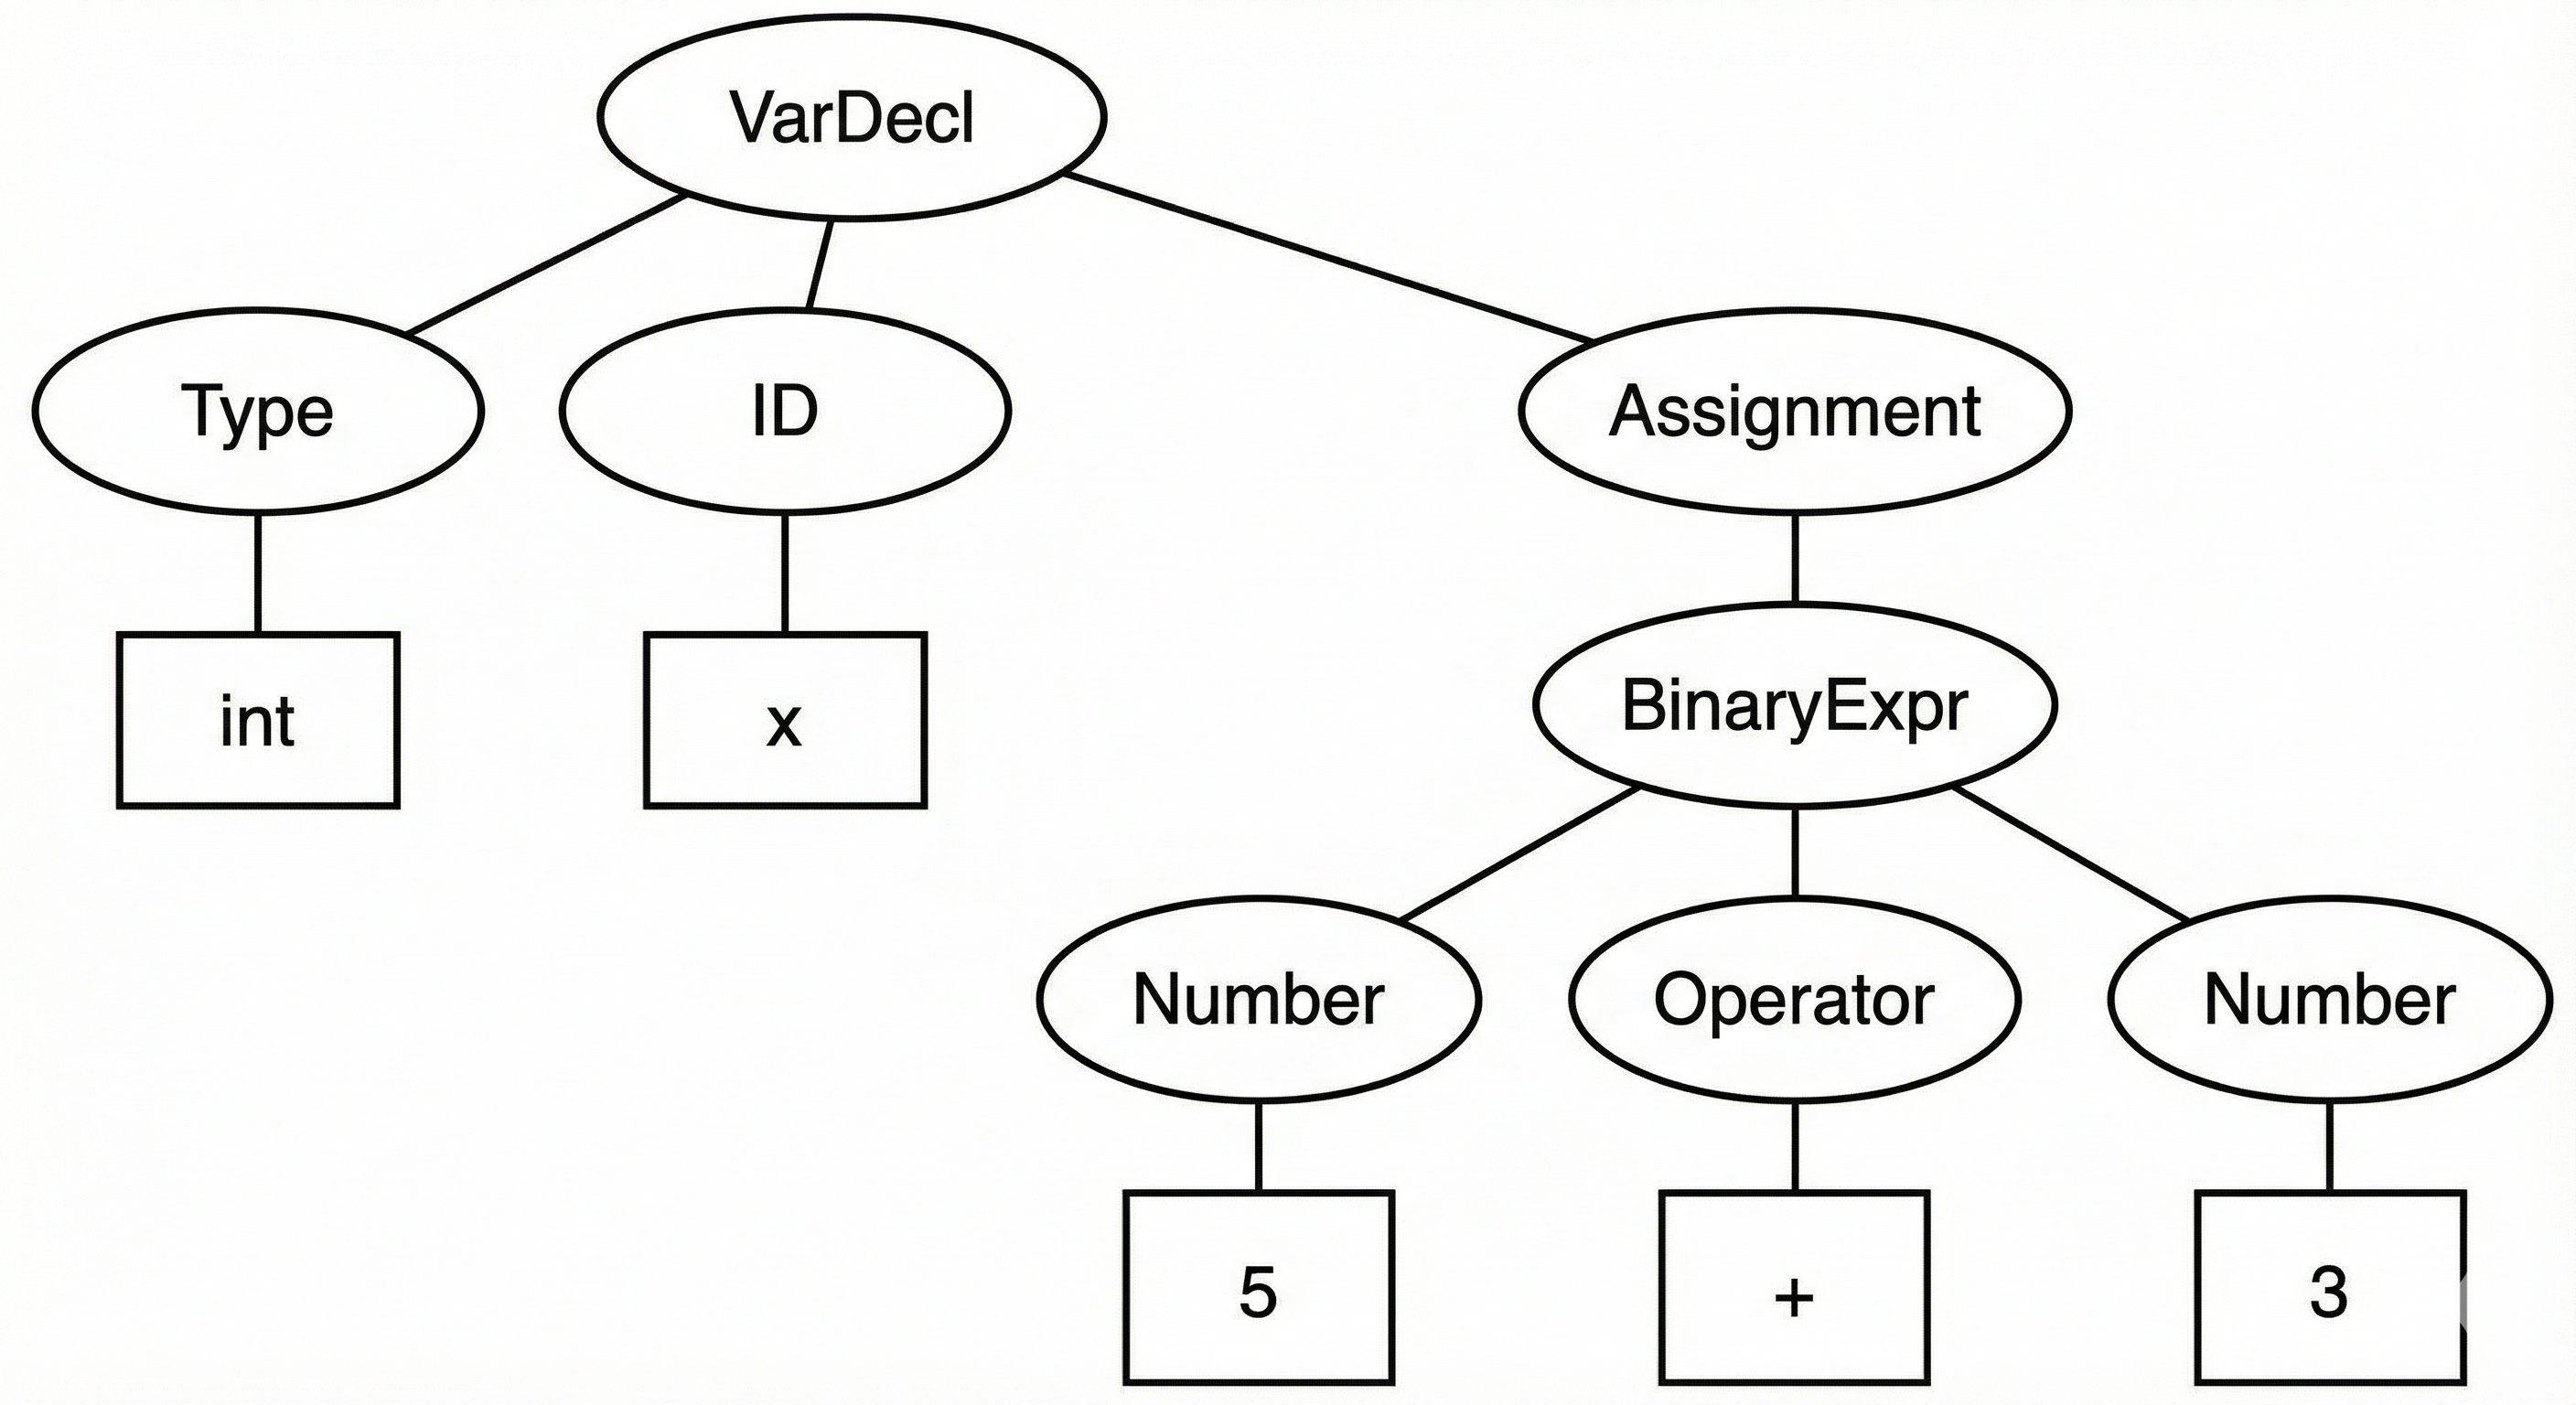
\includegraphics[width=\textwidth]{parse_tree_example.png}
\caption{Parse Tree for Variable Declaration}
\end{figure}

\subsubsection*{Explanation}
The parse tree represents the hierarchical syntactic structure of the statement `int x = 5 + 3;`. The root node `VarDecl` branches into the type `int`, the identifier `x`, and an `Assignment` node, which further decomposes into a binary expression.

%================================================
\subsection*{DFA 3: AST Traversal Architecture}

The DFA for AST traversal is defined as:

\[
M_3 = (Q, \Sigma, \delta, q_0, F)
\]

\begin{itemize}
    \item \textbf{State set}
    \[
    Q = \{q_{\text{prog}}, q_{\text{class}}, q_{\text{method}}, q_{\text{stmt}}, q_{\text{expr}}, q_{\text{done}}\}
    \]

    \item \textbf{Alphabet} $\Sigma = \{\text{AST Nodes}\}$

    \item \textbf{Transition function} $\delta : Q \times \Sigma \rightarrow Q$

    \item \textbf{Initial state} $q_0 = q_{\text{prog}}$

    \item \textbf{Final state set} $F = \{q_{\text{done}}\}$
\end{itemize}

\begin{figure}[H]
\centering
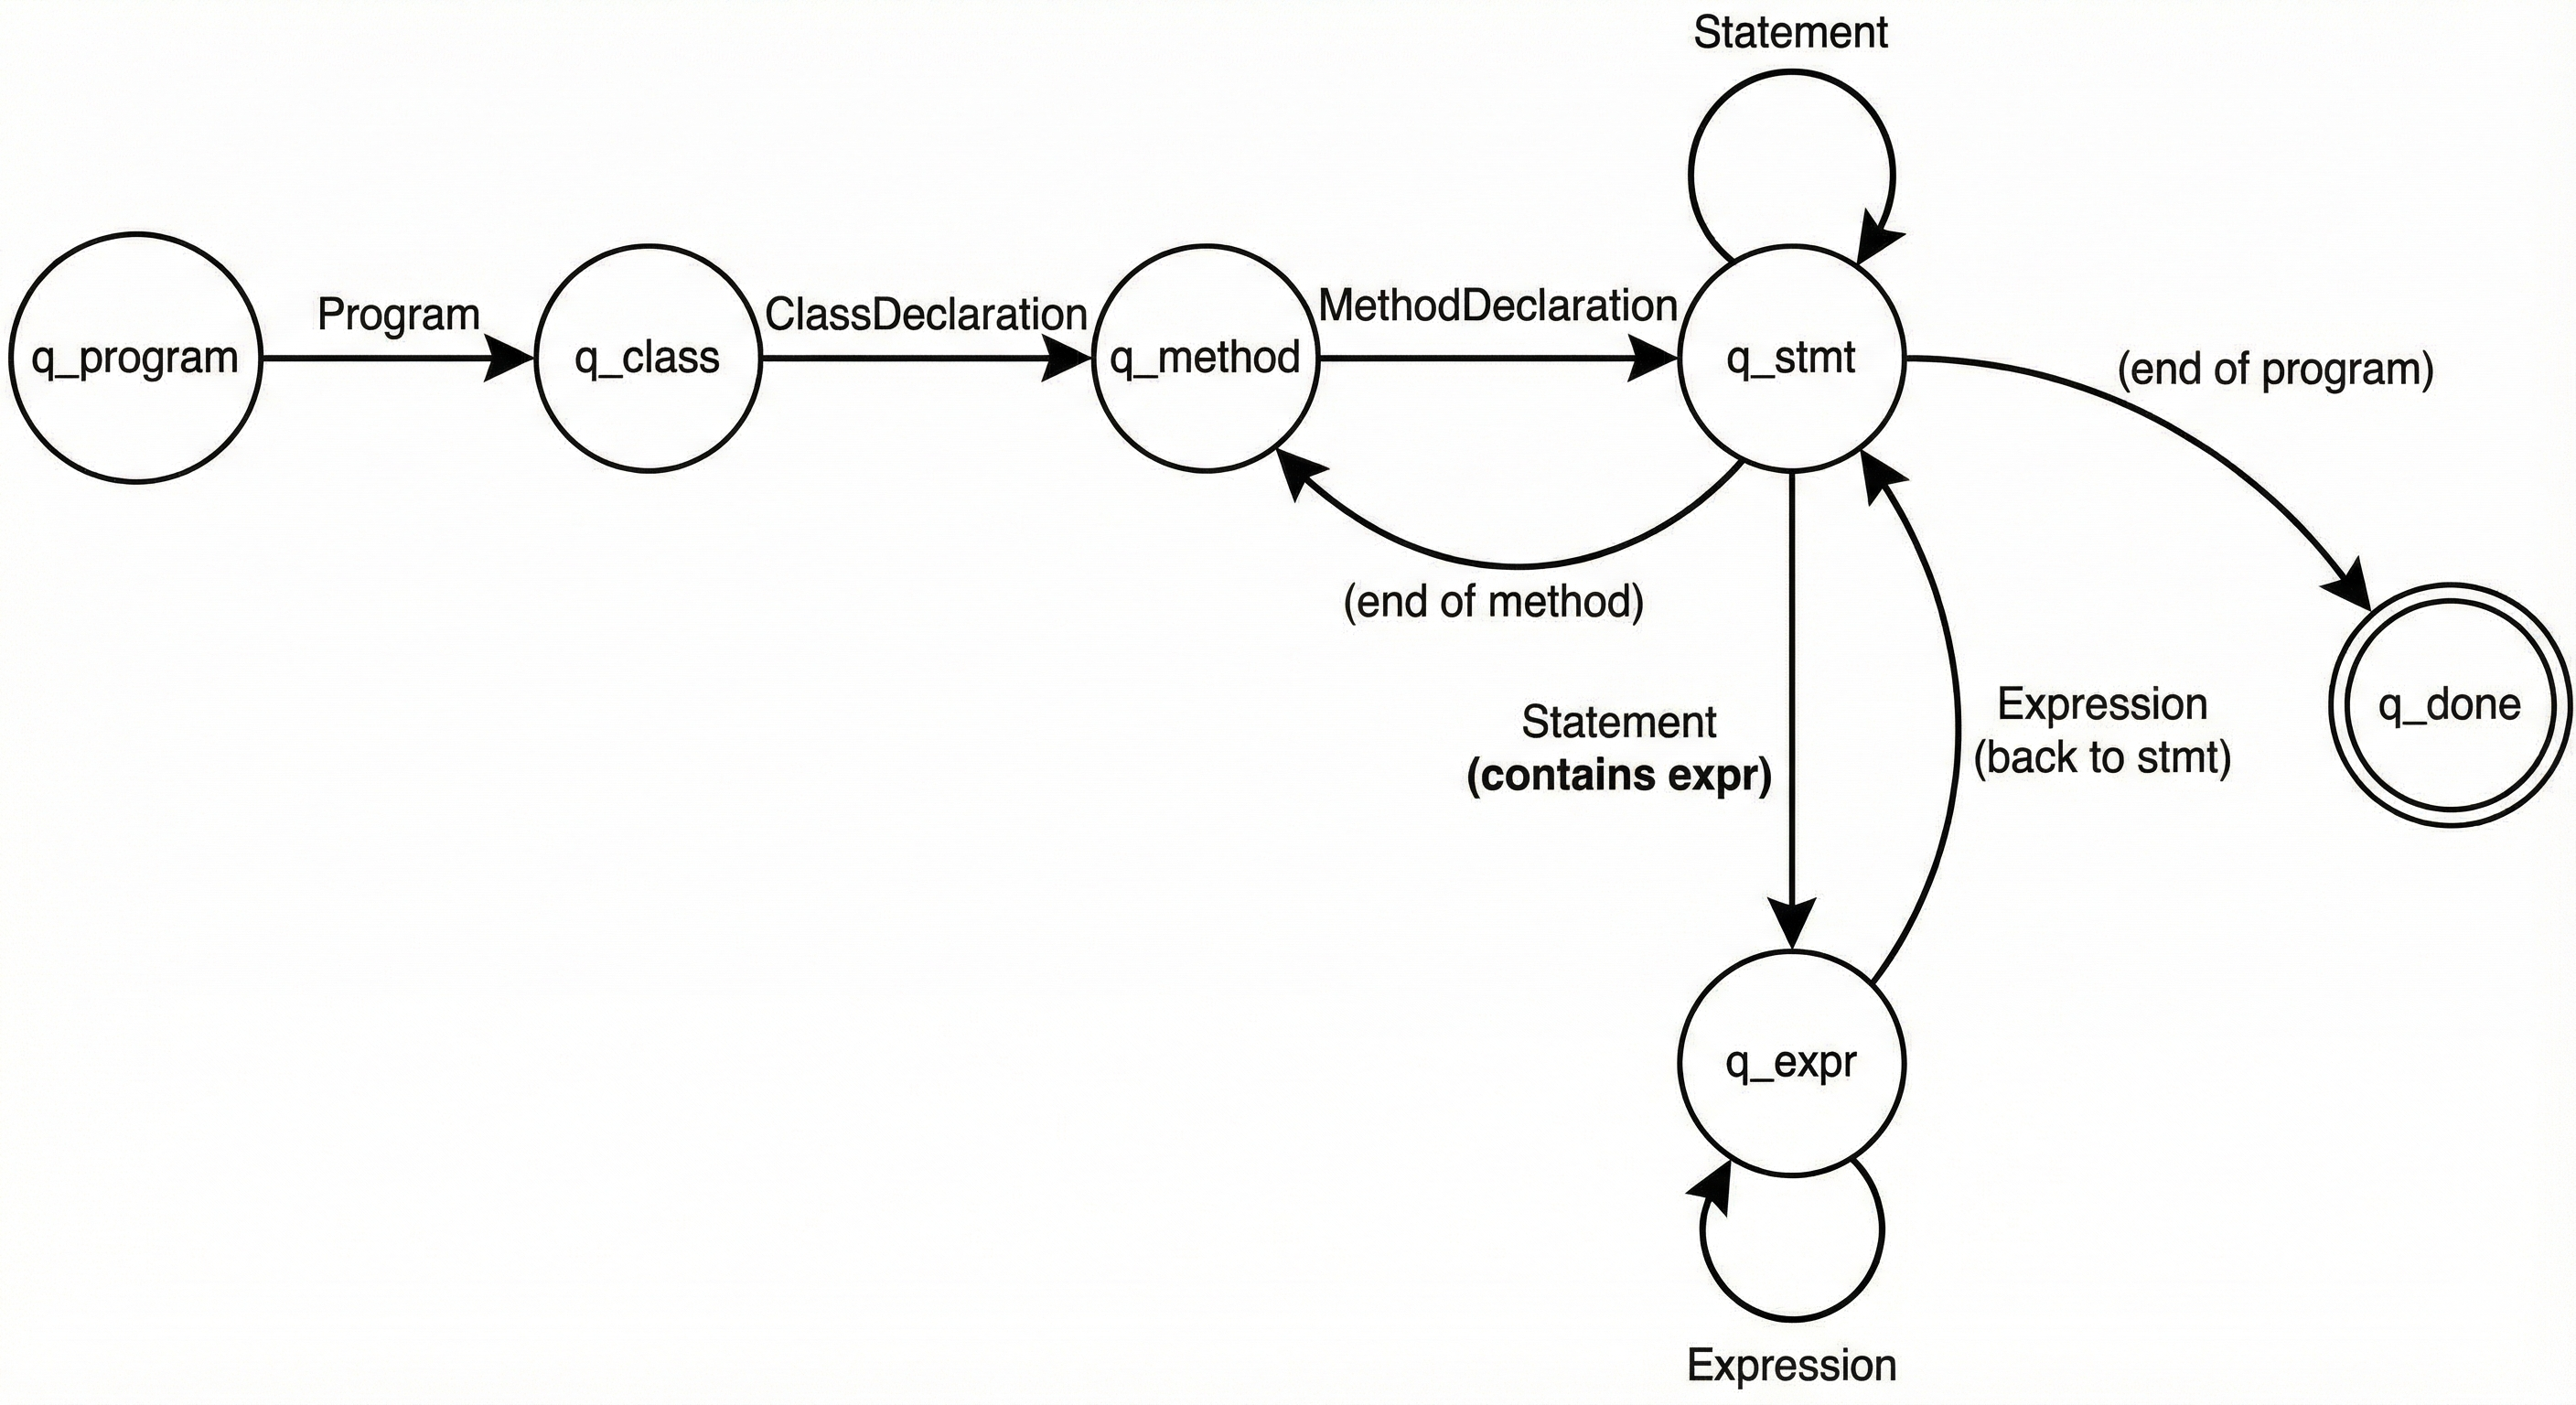
\includegraphics[width=\textwidth]{dfa3_ast_traversal.png}
\caption{DFA 3: AST Traversal State Machine}
\end{figure}

\subsubsection*{Transition Table}

\begin{table}[H]
\centering
\begin{tabular}{|c|c|c|}
\hline
Current State & Visit Node & Next State \\
\hline
$q_{\text{prog}}$ & Program & $q_{\text{class}}$ \\
$q_{\text{class}}$ & ClassDecl & $q_{\text{method}}$ \\
$q_{\text{method}}$ & MethodDecl & $q_{\text{stmt}}$ \\
$q_{\text{stmt}}$ & Statement & $q_{\text{stmt}}$ or $q_{\text{expr}}$ \\
$q_{\text{stmt}}$ & End of Block & $q_{\text{method}}$ \\
\hline
\end{tabular}
\end{table}

\subsubsection*{Tree Grammar}

The grammar is defined as:

\[
G_3 = (V, T, P, S)
\]

\begin{itemize}
    \item \textbf{Variable set}
    \[
    V = \{Program, Class, Method, Stmt\}
    \]

    \item \textbf{Terminal set} $T = \{NodeTypes\}$

    \item \textbf{Start symbol} $Program$

    \item \textbf{Production rules}
    \[
    Program \rightarrow Class^+
    \]
    \[
    Class \rightarrow Method^*
    \]
\end{itemize}

\subsubsection*{Explanation}
This DFA models the traversal of the Abstract Syntax Tree (AST) using the Visitor pattern. The state machine moves through the hierarchical structure of the code, visiting nodes in a depth-first manner. This traversal is crucial for semantic analysis and code generation, ensuring that every part of the program is processed in the correct context.

%================================================
\subsection*{DFA 4: Code Generation Architecture}
The DFA for code emission is defined as:

\[
M_4 = (Q, \Sigma, \delta, q_0, F)
\]

\begin{itemize}
    \item \textbf{State set}
    \[
    Q = \{q_{\text{pkg}}, q_{\text{imp}}, q_{\text{type}}, q_{\text{func}}, q_{\text{body}}, q_{\text{end}}\}
    \]

    \item \textbf{Alphabet} $\Sigma = \{\text{AST Nodes}\}$

    \item \textbf{Transition function} $\delta : Q \times \Sigma \rightarrow Q$

    \item \textbf{Initial state} $q_0 = q_{\text{pkg}}$

    \item \textbf{Final state set} $F = \{q_{\text{end}}\}$
\end{itemize}

\begin{figure}[H]
\centering
\includegraphics[width=\textwidth]{dfa4_codegen_emission.png}
\caption{DFA 4: Code Emission State Machine}
\end{figure}

\subsubsection*{Transition Table}

\begin{table}[H]
\centering
\begin{tabular}{|c|c|c|}
\hline
Current State & Action & Next State \\
\hline
$q_{\text{pkg}}$ & Emit Package & $q_{\text{imp}}$ \\
$q_{\text{imp}}$ & Emit Imports & $q_{\text{type}}$ \\
$q_{\text{type}}$ & Emit Struct & $q_{\text{func}}$ \\
$q_{\text{func}}$ & Emit Receiver & $q_{\text{body}}$ \\
$q_{\text{body}}$ & Emit Stmt & $q_{\text{body}}$ \\
\hline
\end{tabular}
\end{table}

\subsubsection*{Output Grammar (Go)}

The grammar is defined as:

\[
G_4 = (V, T, P, S)
\]

\begin{itemize}
    \item \textbf{Variable set}
    \[
    V = \{GoFile, TypeDecl, FuncDecl\}
    \]

    \item \textbf{Terminal set}
    \[
    T = \{package, import, type, func\}
    \]

    \item \textbf{Start symbol} $GoFile$

    \item \textbf{Production rules}
    \[
    GoFile \rightarrow Pkg \; Imp \; TypeDecl^* \; FuncDecl^*
    \]
\end{itemize}

\subsubsection*{Explanation}
This DFA represents the final stage of the compiler: code generation. It models the sequential emission of Go code constructs. The state machine ensures that the generated code follows the structure of a valid Go program (package declaration, imports, types, functions). The transitions correspond to the `emit` operations in the `CodeGenerator` class.

%------------------------------------------------

\newpage
\section*{Conclusion}

This case study demonstrates that automata theory provides a rigorous and systematic framework for modeling, analyzing, and implementing a compiler. By representing the phases of the J2GO transpiler as Deterministic Finite Automata, we can verify the correctness of the translation process. The use of multiple DFA representations illustrates the different levels of abstraction required in a compiler, from character-level tokenization to tree-level code generation. This work establishes a clear connection between formal automata theory and practical software engineering in compiler construction.

\end{document}
